 \begin{frame}
  \frametitle{Mission}
  
  \begin{block}{Matériel}
   \begin{itemize}
    \item Eléments de base LEGO
	  \uncover<2->{
    \item Capteurs}
	  \uncover<3->{
    \item Moteurs}
	  \uncover<4->{
    \item Damier blanc/gris + feuilles noires pour les obstacles}
   \end{itemize}
  \end{block}

  \uncover<5->{
  \begin{block}{Objectif}
   \begin{itemize}
    \item Progression du maître dans le "labyrinthe" (succession de comportements de base)
	  \uncover<6->{
    \item Communication des ordres à l'esclave}
	  \uncover<7->{
    \item Atteinte de la sortie}
   \end{itemize}
  \end{block}
  }

 \end{frame}

 \begin{frame}
  \frametitle{Le Damier - justification}
 \center
  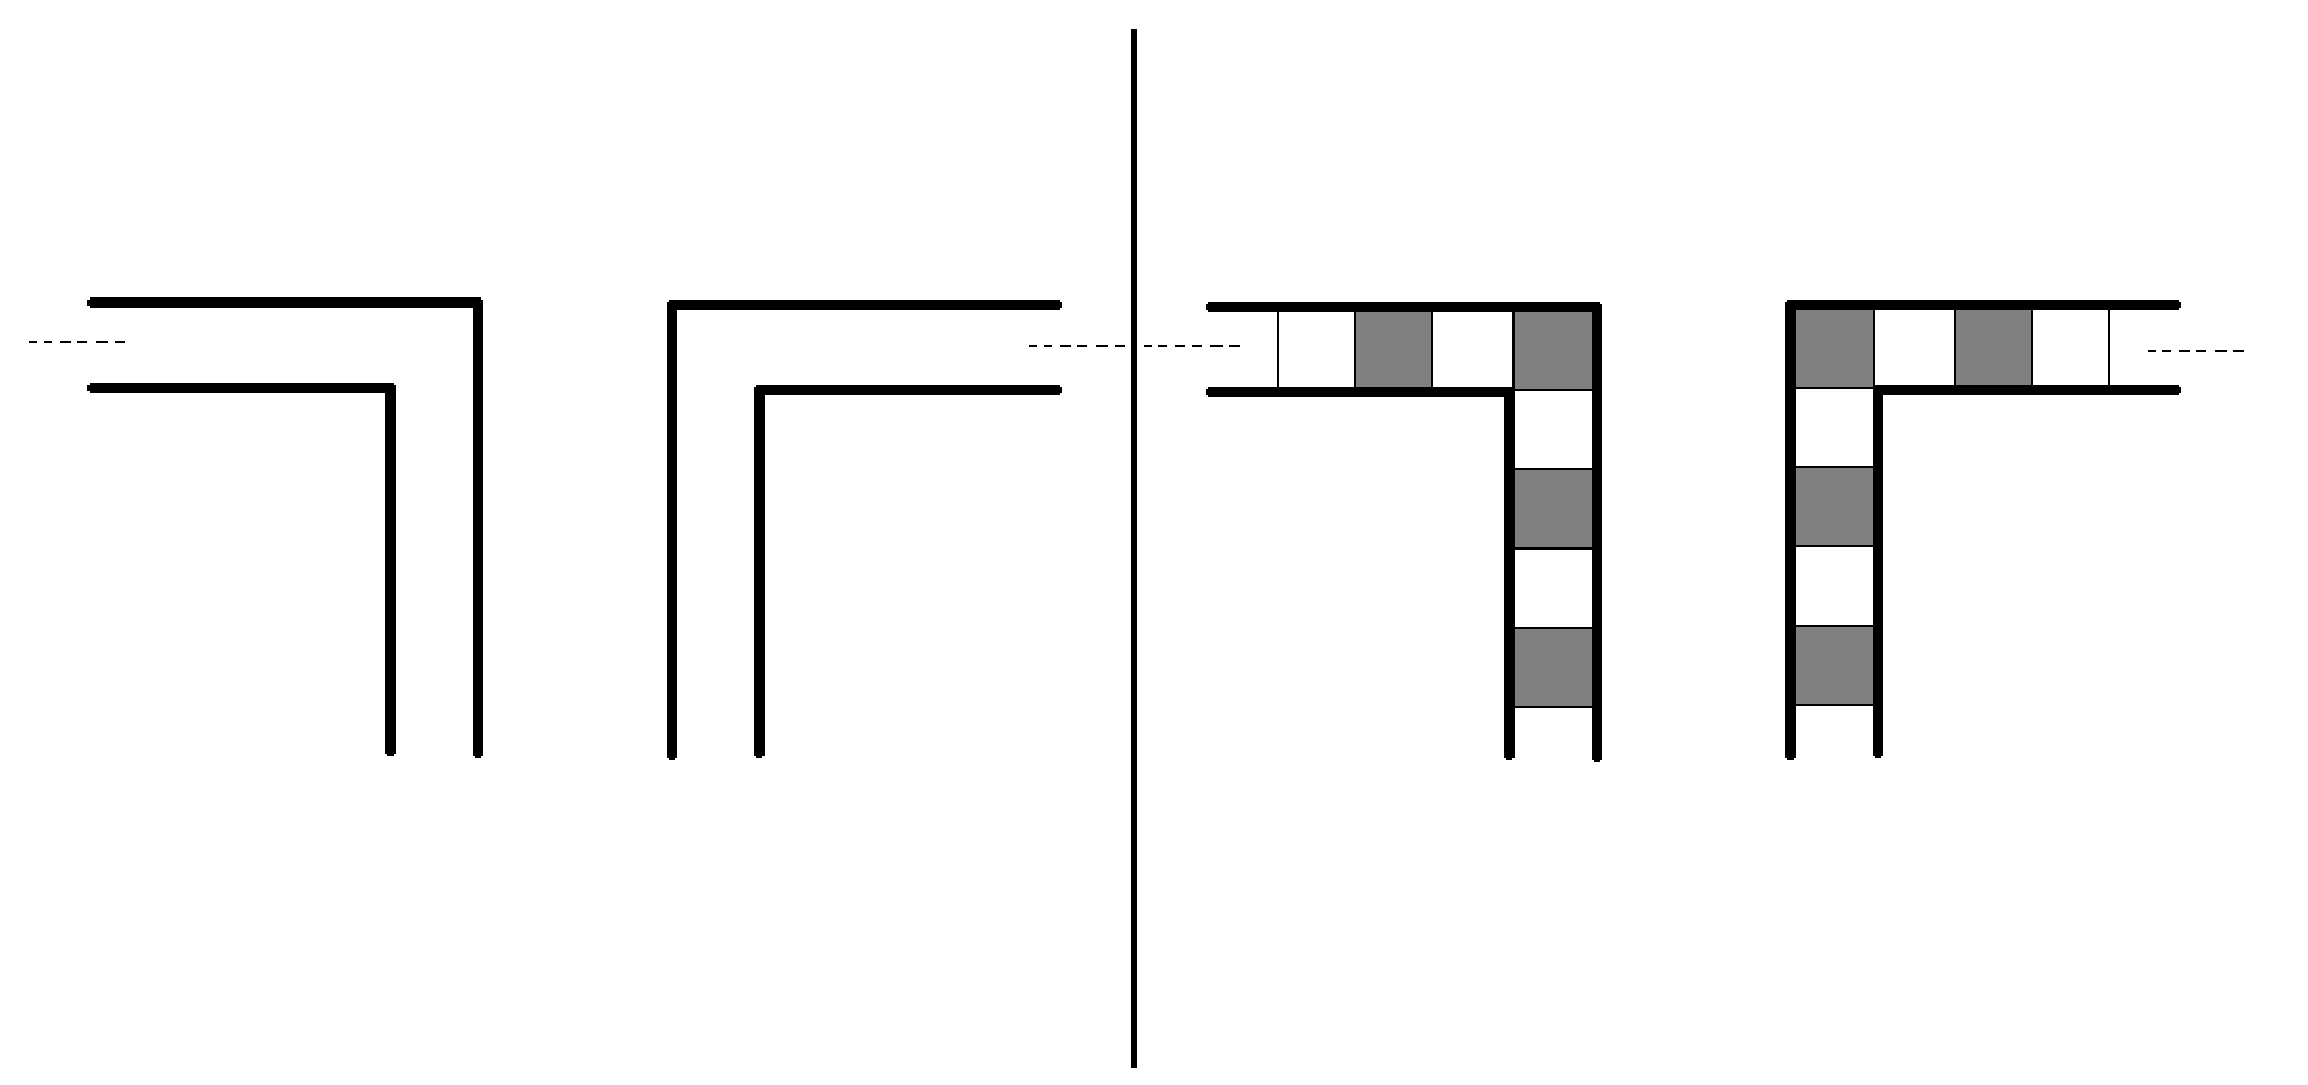
\includegraphics[height=5cm]{damier.eps}
  \end{frame}
